\documentclass[11pt]{article}
\usepackage[margin=0.75in]{geometry}
\usepackage{hyperref}
\usepackage{graphicx}
\usepackage{float}
\graphicspath{ {images/} }

\title{fMRI Dataset from Complex Natural Simulation with \emph{Forrest Gump}: \\A Restudy}
\author{
  Chang, Jordeen\\
  \texttt{jodreen}
  \and
  Daks, Alon\\
  \texttt{AlonDaks}
  \and
  Luo, Ying\\
  \texttt{yingtluo}
  \and
  Yu, Lisa Ann\\
  \texttt{lisaannyu}
}

\bibliographystyle{siam}

\begin{document}
\maketitle

\abstract{Most fMRI studies use highly simplified stimuli that are very
different from what people experience in everyday life. ``A High-Resolution 7-Tesla fMRI Dataset from Complex Natural Stimulation with an Audio Movie" by
Hanke et al. sought to create a dataset of naturally occurring brain states
by exposing participants to a more complex stimulus, the audio description of
\emph{Forrest Gump}. Scanning subjects who are listening to the two hour audio track of the movie allows for the study of
auditory attention and cognition, language and music perception, and retrieval
of explicit memory without the effect of visual imagery. Furthermore, the
study was conducted on 20 subjects enabling research into brain similarities
among individuals when exposed to the same complex stimulus. The goal of our
paper is to first reproduce a subset of the analysis conducted by Hanke et al. where we will analyze inter-subject correlation among 5 subjects, then apply machine learning to see if we can predict if a subject was
listening to an interior or exterior scene of the movie based on brain state. The results for our reproduction are consistent with those produced by Hanke et al. and our internal-external scene classifier has a validation accuracy of 0.934.}

\section{Introduction}

The main purpose of the original study was to examine properties of brain
response patterns that are supposedly common when people are exposed to audio
and movie stimulation, since that should be more representative of naturally 
occurring brain states than highly simplified experiments with a simple on/off
stimulus.  Additionally, the literature is almost entirely limited to visual 
stimulation, which is why Hanke et al. chose to use an auditory version of 
\emph{Forrest Gump} produced for a visually impaired audience. 

We intend to replicate their experiment using the data
they gathered from the 20 participants. For example, a BOLD time-series
similarity measure (e.g. correlation) is often used to quantify similarities
in responses among individuals. Hanke et al. recognized that this was a common
approach, but went beyond that by implementing a representational
similarity analysis (RSA)\cite{hank2014audiomovie}. To replicate their 
analysis, we will calculate inter-subject pairwise correlations among 5 individuals.
Lastly, to access statistical significance, we will transform the 
representational consistency map into percent rank with respect to the total 
distribution of the DSM correlations. We'll calculate both the pooled and mean 
correlation coefficients and compare our values to theirs.

We intend to extend their experiment by adding a classification analysis that
predicts which scenes take place inside and which take place outside.  We will
select voxels with the largest difference in BOLD signal
between interior and exterior scenes to be our features, then use random forest to 
predict volumes as interior or exterior.

Before we formally began, we performed basic sanity checks on the data. We
downloaded and loaded the files successfully, and we have confirmed that we
have data for every test subject. 

Reproducibility is crucial in research, especially when such high volumes of
data are involved, because it allows other people to fact-check the work. When
people collaborate, new insights can be shed and the rate of progress is
expedited. For this study, we began by extracting data we saw fitting and
asking questions that were not addressed by the original study. To answer
these questions, we utilized neuroscience concepts, additional packages, and
parallel processing techniques. We found that in certain functions, such as
parsing through csv files, it would have been easier to hard code in the
correct values. However, hard coding would have defeated the reproducibility
aspect of our study because our code would break if the data were slightly
modified.

A central theme of the course is exploring reproducible practices while 
conducting scientific research. For our project we address reproducibility from 
two perspectives: 1) We attempted to 
reproduce some of the results cited in the original paper by emulating Hanke 
et al.'s technique and comparing values. 2) We designed our code and scripts to be modular and 
portable so that anyone with an appropriate computer can rerun our analysis 
and reproduce the results we cite in this paper. 

\section{Data}

The data is curated and segmented by subject and run. Each subject includes fMRI data along with cardiac and
respiratory trace, angiographies, and structural MRI data. Each subject's fMRI
data includes several formats: raw BOLD functional MRI, BOLD functional
MRI (with applied distortion correction), BOLD functional MRI (linear
alignment: affine transformation), and BOLD functional MRI (non-linear
alignment: affine transformation and non-linear warping). The corrected and aligned versions of the data attempt to
eliminate device and scan related noise. Scan data is accessible in nibabel
compatible formats (.NII).

In addition to data for each subject, there was also data about the
experiment as a whole, including a German audio description of the stimulus
and a csv file with scene information, including the timestamp of the
beginning of each scene, the scene location, whether the scene took place
during the day or night, and whether the scene was interior or exterior.  

The original scenes file contained an error: one scene was labeled `DAY' for 
the interior/exterior column.  We contacted Hanke via Github issue, and he told us the correct 
label was `EXT' for that scene.  

\subsection{Selecting the Data}
Because there were various versions of the
data (e.g. linear vs. non-linear), we had to first isolate which dataset best
suited our needs. The non-linear alignment had more smoothing than the linear
alignment, which made that dataset more appropriate for initial exploratory
data analysis.  We recognize that the non-linear alignment is crude, since it
probably was conducted with no specific hypothesis about which parts of the
brain should be expanded or compressed, but not having the machinery or
background to better preprocess the data, we at first simply used the non-linear
alignment version of the data provided by Hanke et al.
\cite{hank2014audiomovie}.

However, after talking to Matthew Brett about the following plots, 
we decided to use the data kindly preprocessed by Russ Poldrack and the OpenfMRI
group.  These plots show there may be an artifact in the data.  This image shows
the day/night regressor (as explained in the Classification section) and seems
to indicate great activation in the scalp.  Furthermore, it looks remarkably like the linear drift regressor, which also shows a white ring along the scalp
next to a black region, suggesting that the participant moved backwards and to
the left and that Hanke et al.'s preprocessed data could be better motion-corrected.
\begin{figure}[H]                                                               
\caption{Day/Night Regressor}                                                   
\centering                                                                      
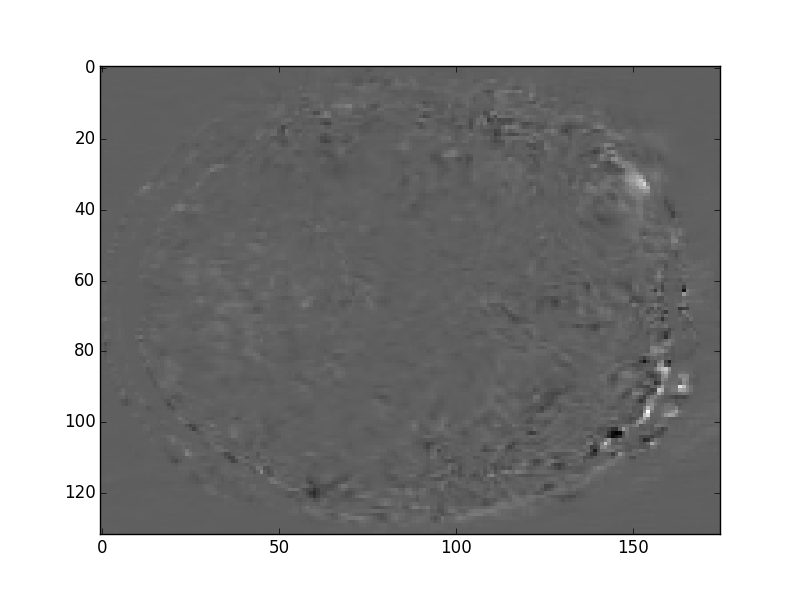
\includegraphics[height=8cm]{day_night_artifact.png}                            
\end{figure}   

\begin{figure}[H]                                                               
\caption{Linear Drift Regressor}                                                   
\centering                                                                      
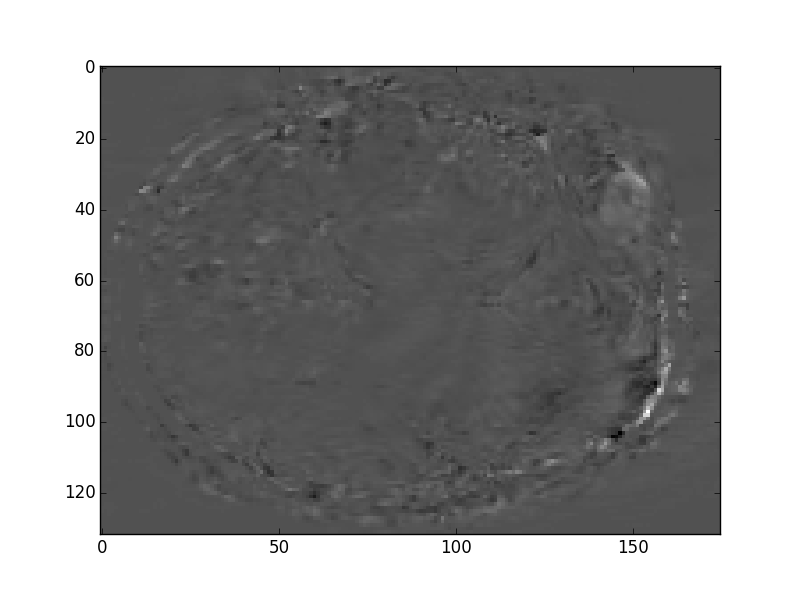
\includegraphics[height=8cm]{linear_drift_artifact.png}                            
\end{figure}  
After reading how Hanke et al. corrected for motion, namely, adjusting the 
scanner itself when participants moved, instead of modeling for their motion, 
which is less prone to error, Matthew suggested we use the preprocessed data
provided by the OpenfMRI group, 
which corrects for motion using a high-pass filter.
   
\subsection{Preprocessing Data}             
fMRI data is noisy, so preprocessing is essential.  In fact, without preprocessing, 
we cannot make any meaningful inferences, since we could be making inference on 
the noise, not the BOLD signal.  There are many sources of noise in fMRI data in general:
activation from outside the brain, subject motion, subject physiology (i.e. heart 
rate and respiration), and scanner noise.  We corrected for activation from outside the brain using a brain mask, as described below.  Poldrack and the OpenfMRI group 
preprocessed the data by correcting for motion, removing low frequency drifts/noise, and registering the data to a standard anatomical template (the MNI template).  We 
also corrected for motion over and above this preprocessing for the classification
analysis by including a linear drift term in our deisgn matrix.
Additionally, there were some sources of noise specific to our dataset, like
having 8 runs per subject, which we corrected for as described below.

\subsubsection{Brain Mask}
In order to be certain we were only looking at BOLD signal from inside the subject's
brain (since we are interested in imaging the brain), we created a brain mask. Looking at only subject 1, we plotted 
the mean volume over time as a histogram and selected a threshold 
of 150 to select for voxels that are inside the brain.
\begin{figure}[H]                                                               
\caption{Mean Volume Over Time for Subject 1}                        
\centering                                                                      
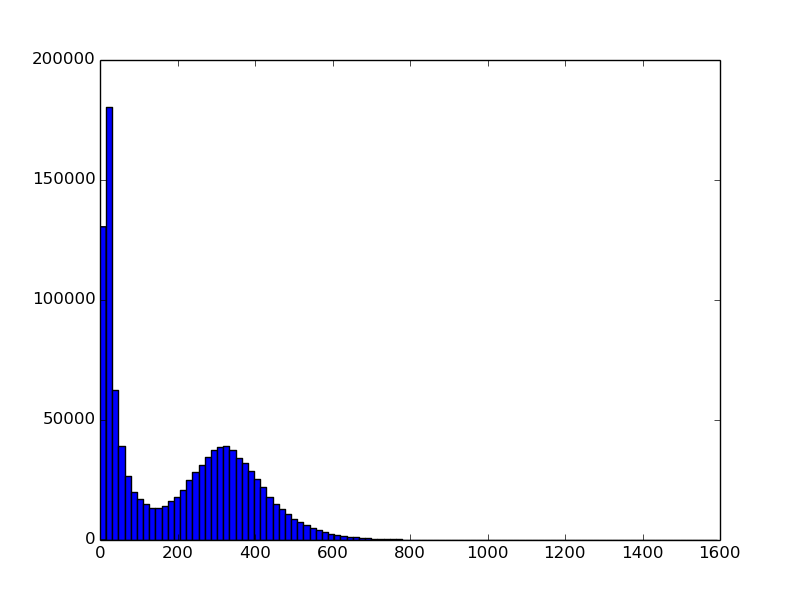
\includegraphics[height=8cm]{subj_1_vol_mean_histogram.png}   
\end{figure}  
There is no clear-cut boundary here, as there are voxels with moderate degrees of activation in the 100-200 range, but we selected 150 because 1) it seems to be the
lowest point between those two peaks at around 30 and 300, and 2) it is in the middle
of that 100-200 range.  When we plot our brain mask, it 
looks like that threshold has done a good job of selecting voxels within the brain. 
\begin{figure}[H]                                                               
\caption{Brain Mask Using Data from Subject 1}    
\centering                                                                      
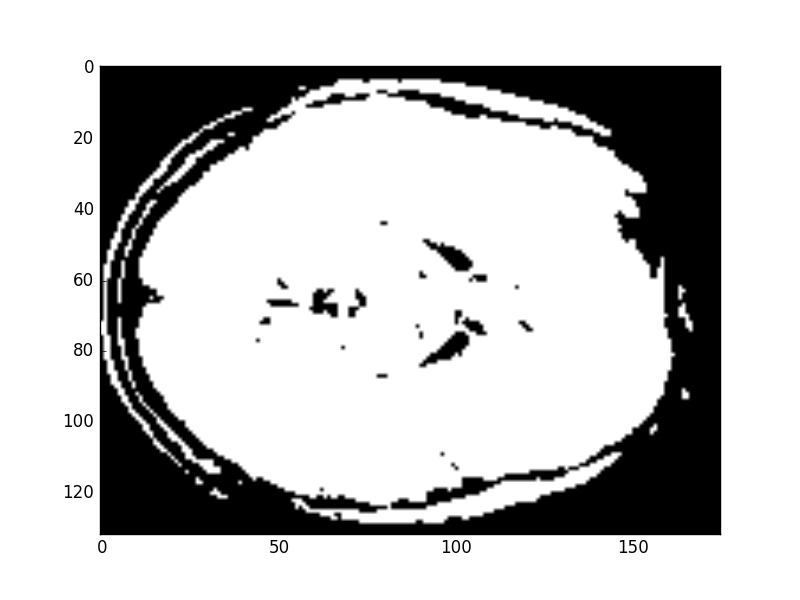
\includegraphics[height=8cm]{brain_mask.png}                            
\end{figure}  
We chose to use subject 1 to generate the brain mask for a few 
reasons.  1) The classification analysis will only be looking at subject 1, so we wanted to be sure we evaluated all the voxels in the brain for that analysis.  2) Since the data provided by Poldrack and the OpenfMRI project 
group preprocessed all the data by registering it to a standard anatomical 
template, we made the assumption that the brain mask for one subject 
should work for all the subjects. Therefore, when calculating voxel-wise correlations between pairs of subjects, we only consider voxels that are within the brain region according to the mask generated by subject 1.

\subsubsection{Concatenating Across Runs}
Due to the length of the movie, the stimulus was split up into eight runs,  
each approximately fifteen minutes long. The participants listened to four  
runs on two separate days of fMRI scanning.  At every        
run boundary except for the first, Hanke et al. repeated at least the last 
six seconds of movie audio between the beginning and end of each segment so there would be a 
short stimulus overlap between runs. In the original analysis, they removed the first and last four 
volumes of the data connecting each run, presumably to account for the overlap 
between segments, although it is not entirely clear from their article. Consequently, for our analysis we also removed the first and last four 
volumes of the data connecting each of the eight runs and concatenated the data into a single file. 

\subsubsection{Smoothing}
We smoothed the data spatially before performing any analyses by applying a Gaussian      
filter. There are two main motivations for spatial smoothing: first a spatial Gaussian
filter smooths the signal between adjacent voxels, addressing                   
our assumption that neighboring voxels are not independent. Since the original scans were conducted at very high, 7-Tesla resolution, smoothing mitigates IID scanner noise across voxels. Second, spatial smoothing addresses the concern that subjects’ brains are not anatomically the same shape. The effects of small differences in brain shape can be reduced by smoothing since as the brain becomes blurrier, precise shape differences between subjects become harder to discern. The Gaussian filter from the scipy.ndimage module smooths the data in terms of voxel standard deviations, however it is conventional in fMRI studies to smooth in terms of millimeter full-width-half-maximum (FWHM).  Therefore, we first had to convert mm FWHM into mm SDs, and then convert mm SDs into voxel SDs by computing the width of each voxel in millimeters in all three directions from the affine transformation.

We produced two versions of smooth data, one for the reproduction analysis, and
the other for the classification analysis.  We smoothed using 8 mm in FWHM along each axis
for the reproduction analysis, and 4 mm in FWHM along each axis for the classification
analysis.  For the reproduction analysis, we are taking correlations between
subjects, so we need to smooth more to adjust for brain shape differences. For the classification analysis, we just want to smooth out scanner noise, so we applied a more conservative filter. The intuition for using 8mm and 4mm respectively was provided by JB Poline, a domain expert.

Note: smoothing does not take treat edge voxels any differently from voxels in the 
interior of the brain.  Therefore, some voxels outside the brain will be activated.  
According to Ross Barnowski and Matthew Brett, who we contacted via Github issue, 
this is not a huge issue, and in fact, most brain imaging studies ignore this 
problem.  The brain mask also mitigates the issue, since we have already selected 
for only the voxels that are inside the brain.

\subsubsection{Reshaping}
Once we have preprocessed the data by concatenating the data and smoothing it,
we reshape it to a 2D array: number of voxels (1,108,800) by time (3543). Working with a flattened matrix allows us to vectorize correlations between subjects and takes the form of the transpose of the design matrix for classification.  

\section{Reproduction}

\subsection{Methods}

The original paper focused on inter-individual response pattern similarity. In
other words, their analysis measures brain pattern correlation between
subjects who listened to \emph{Forrest Gump}. Hanke et al. identifies two 
methods for measuring correlation. The first method takes the BOLD time-series 
and calculates the voxel-wise Pearson correlation and the second method employs
``representational similarity analysis to identify 2nd-order isomorphisms in
the response patterns across brains"\cite{hank2014audiomovie}.  Since the first 
technique is simpler, we chose that to be the portion of the analysis we tried 
to reproduce. 

\subsubsection{Data}
Although 20 subjects were scanned, Hanke et al. excluded subjects 4 and 10 
from their correlation analysis because some data for those two subjects is missing\cite{hank2014audiomovie}. With the 18 
remaining subjects there are 153 pairs (18 choose 2) for which voxel-wise 
correlations are calculated. Hanke et al. calculated correlations on linearly 
and non-linearly aligned raw data. Additionally both versions of the raw data were applied through a bandpass filter. Hanke et al. did not perform Gaussian smoothing on their data. 

For our reproduction, we are using 8 mm FWHM smoothed data as described in the preprocessing section of this paper. As a reminder to the reader, this data has been passed through a high-pass filter and is non-linearly aligned in addition to the smoothing we conducted ourselves. Because of memory and storage limitations, we decided to only calculate 
correlations between five subjects: subjects 1-3 and 5-6, since subject 4 
had missing data, as noted above.  In addition, we wanted to pick 5 
subjects who were representative of the general population.  These five 
subjects include both males and a female, and subjects in the 20-25, 25-30,
and 30-35 age brackets, which is relatively diverse for this sample.

Our fMRI data measures BOLD signal, not the neural signal itself, and it takes
some time for the blood oxygenation to change once a scene has changed.  To 
compensate for this delay, we removed the first 2 volumes after each flip from 
` `Interior" to ` `Exterior" or vice versa, a total of 4 seconds, since our TR is 2 
seconds.  For example, the first scene takes place in the savannah (outside), and the second takes place in the doctor's office (inside).  The scene in the doctor's office
started at 272 seconds, so we removed the first four, and only looked at the BOLD
signal starting from 276 seconds.

\subsection{Analysis}
With 5 subjects, we have 10 pairs (5 choose 2) 
in total rather than the 153
(18 choose 2) pairs Hanke et al. used for calculating inter-subject correlation.  Although we reduced to 5 subjects because of system constraints, we believe that working with 5 subjects should still yield results consistent with those published by Hanke et al.
Thus, our voxel-wise inter-brain correlation was determined for 10 pairs as the 
Pearson correlation of the time courses for each voxel, yielding a total of 1,108,800 (number of voxel) correlation values for each subject pair.
Hanke et al. reported values for the pooled and mean voxel-wise inter-individual correlation at various percentiles for both the linear and 
non-linear anatomical alignments. `Pooled' correlation values are found by taking the union of all 1,108,800 correlations from each subject pair, yielding 11,088,000 values whereas `mean' correlation values average respective voxels, maintaining 1,108,800 values. 

Before continuing with calculating voxel time-course correlations an important caveat must be considered. Taking correlations across the entire 2 hour time-course might be adversely affected by arbitrary run differences. We demonstrate this potential issue via simulation. Suppose we have a voxel time-course for subject a and subject b across 2 runs. Each run contains 100 volumes. Further suppose the values from the first run are distributed iid $Normal(5, 2)$ and values from the second run are distributed iid $Normal(10, 2)$ where subject a's values are independent from subject b's values. The figure below visualizes this simulation.

\begin{figure}[H]                                                               
\caption{Runs Effect Simulation}                                                   
\centering                                                                      
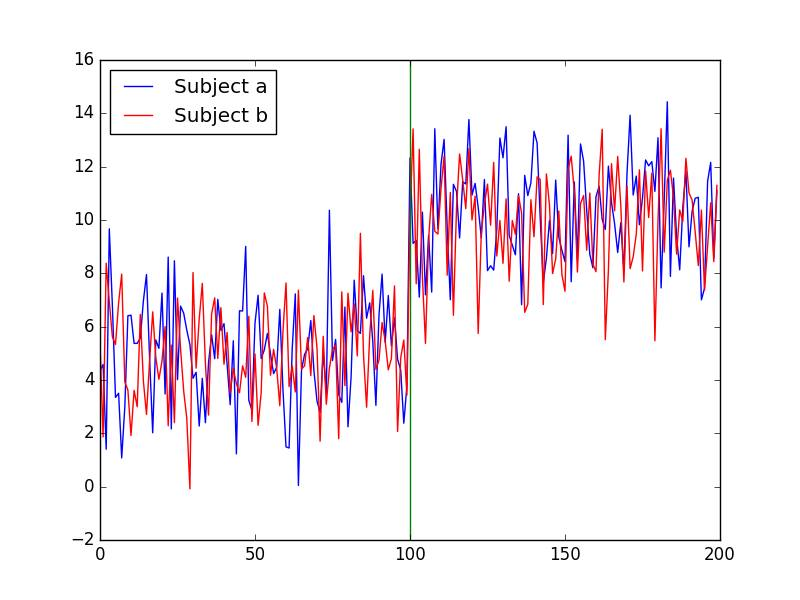
\includegraphics[height=8cm]{simulation.jpg}                            
\end{figure}  

The correlation between the 2 subjects across the both runs is 0.6336, which
seems relatively high. Indeed it would seem to indicate that the subjects' voxels are activated 
roughly the same amount at the same times. However, there is a confounding
factor of the difference in signal between the two runs.  To investigate that
confounding factor, we look at the correlations within each run separately.  
The correlation between the two subjects within the first run is -0.236, and 
the correlation between the two subjects within the second run is 0.0883.  
Thus, the relatively high overall correlation of 0.6336 between the 2 subjects 
is actually a measure of the difference between runs, not the correlation 
between subjects.


Since run segments could arbitrarily affect voxel time-course correlations as shown in the example above, we need to test whether our data does in fact contain arbitrary behavior due to run segmentation. We took our 2D data of voxels by  time (V x T), and took the 
difference between signal from one volume to another, giving us a 2D array of 
V x (T-1), or 1,110,880 by 3542. To get a measure of the signal of the brain at 
every point in time, we took the RMS across all voxels for a particular time to 
get a 1D array of length (T-1), or 3542. Below is the plot of the RMS error for each of the 3542 points using data from subject 1. 

\begin{figure}[H]                                                               
\caption{RMS Error Demonstrating the Runs Effect}   
\centering                                                                      
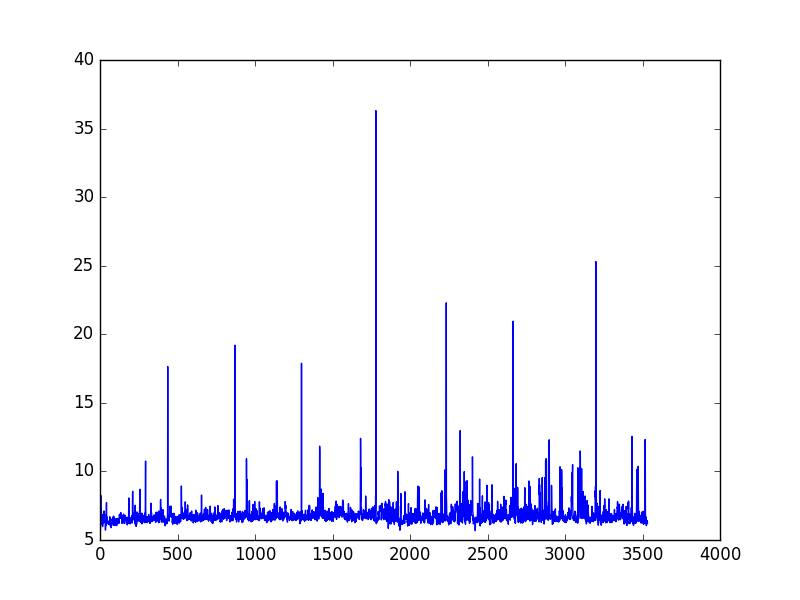
\includegraphics[height=8cm]{runs_effect.jpg}                            
\end{figure}  

There are seven clear spikes, 
representing the seven points between runs.  The highest point is the fourth 
one, which is the point between the first day of fMRI imaging and the second
day.  Thus, it is clear that there is a difference in signal between runs and
we need to correct for it.  

We look to our simulation to find an answer for correcting against the runs affect. If we calculate correlation for a voxel within respective runs and then average those values, we will get more sensible results. Concretely, in our simulation if we average -0.236 and 0.0883, we get a correlation of -0.07385 for the overall voxel time-course, which is much more sensible than 0.6336. Therefore, when calculating inter-subject correlation for a voxel, we will calculate 8 correlations (within respective runs for that voxel) and then average those values together to yield the overall voxel time-course correlation.

To measure our correlation results, will calculated the pooled and mean correlation values and compare our result at the 0, 25, 50, 75, 90, 95, 99, 99.5, 
and 100\% percentiles to that of Hanke et al. In considering percentiles from the set of voxel correlation values, we only look at values from correlations that where within subject 1's brain, as defined by our brain mask, ensuring that we are only reporting on data generated by the brain and not noise. According to
Hanke et al., using this threshold procedure as a measure of statistical 
significance ``has prove to be robust compared to classical testing" \cite{hank2014audiomovie}.

\subsection{Results}
\begin{figure}[H]                                                               
\caption{Pooled Correlation Coefficients}
\centering                                                                      
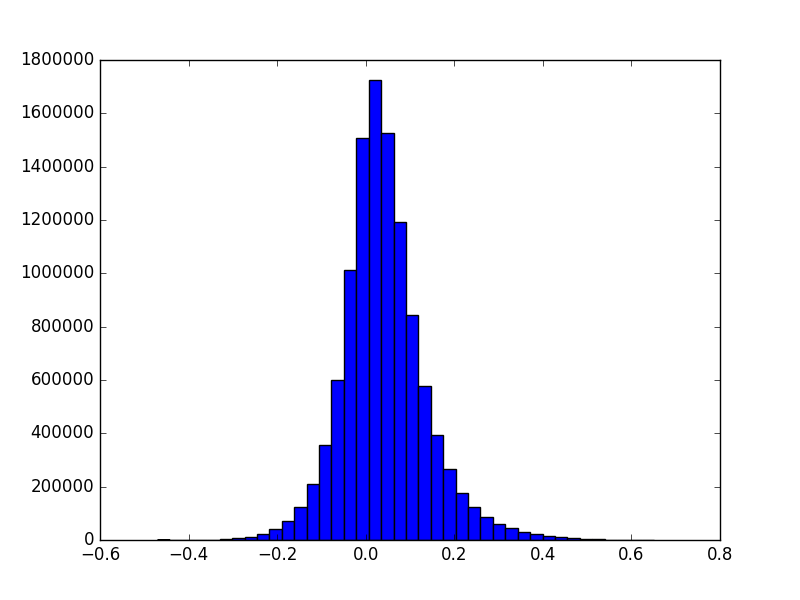
\includegraphics[height=8cm]{pooled_correlation_histogram}
\end{figure}  
\begin{figure}[H]                                                               
\caption{Mean Correlation Coefficients}
\centering                                                                      
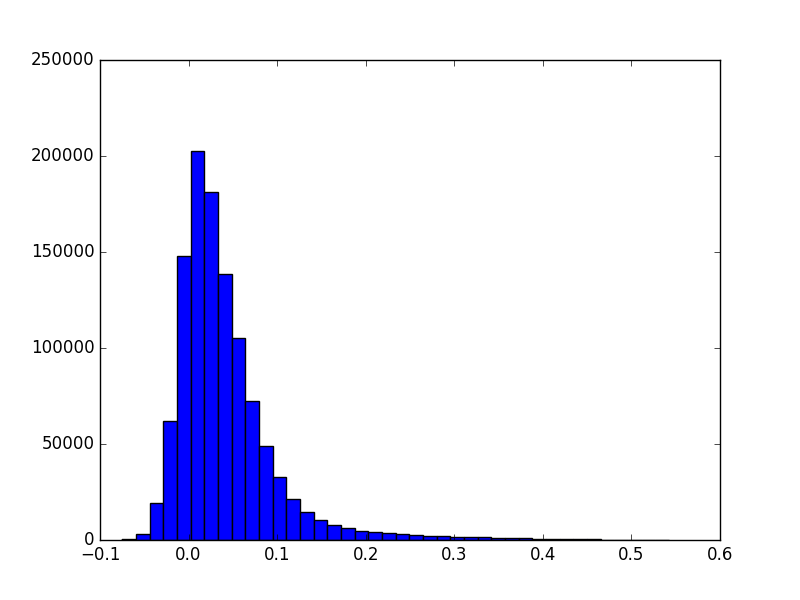
\includegraphics[height=8cm]{mean_correlation_histogram}                            
\end{figure}  

These correlation coefficients are both centered slightly right of
0, which we expect, since we expect there to be a weak inter-subject
correlation for most voxels.

From those correlation coefficient distributions, we calculated the 
correlation coefficients at the 0, 25, 50, 75, 90, 95, 99, 99.5, and 100\%
percentiles, as can be seen in the table below.
\begin{table}[H]
  \centering
  \caption{Our Results}
  \label{tab:table1}
  \begin{tabular}{cccccccccc}
    percentile & 0 & 25 & 50 & 75 & 90 & 95 & 99 & 99.5 & 100\\
    \hline
    pooled & -0.444 & -0.005 & 0.041 & 0.098 & 0.171 & 0.232 & 0.370 & 0.419 & 0.652\\
    \hline
    mean & -0.074 & 0.012 & 0.035 & 0.070 & 0.125 & 0.186 & 0.342 & 0.387 & 0.543\\
  \end{tabular}
\end{table}

\begin{table}[H]
  \centering
  \caption{Results reported by Hanke et al.}
  \label{tab:table2}
  \begin{tabular}{cccccccccc}
    percentile & 0 & 25 & 50 & 75 & 90 & 95 & 99 & 99.5 & 100\\
    \hline
    pooled & {-0.412} & {-0.013} & 0.008 & 0.031 & 0.056 & 0.078 & 0.163 & 0.207 & 0.719\\
    \hline
    mean & {-0.008} & 0.002 & 0.005 & 0.013 & 0.032 & 0.052 & 0.103 & 0.126 & 0.269\\
  \end{tabular}
\end{table}

Our correlations appear to differ slightly from Hanke et al.'s reported numbers.  In 
general, our numbers are higher in magnitude than theirs, but are still within a reasonable distance from theirs.

Once we had that correlation coefficient percentiles, we applied a threshold of 
percentile rank of 95\% to get voxels with a relatively high correlation 
coefficient.  In our data, the 95th percentile corresponds to r = 0.0143 for 
the mean correlation coefficient distribution.  Voxels with a correlation
coefficient above this threshold were coded blue, and all other points 
were coded gray, as shown below.  
\begin{figure}[H]                                                               
\caption{Our Area of Maximum Inter-Brain Time-Series Correlation (at the 95\% level)}
\centering                                                                      
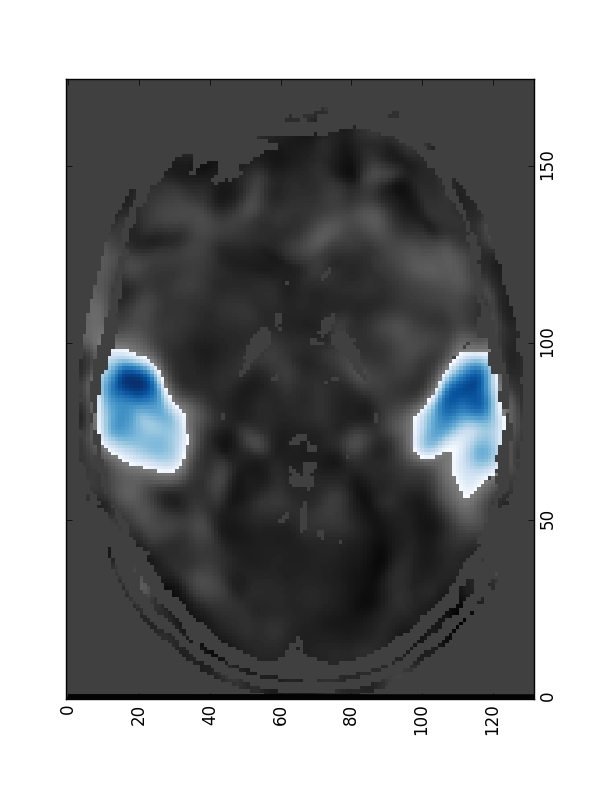
\includegraphics[height=8cm]{correlated_brain.png}                            
\end{figure}  

Hanke et al.'s inter-individual response similarity analysis yielded a similar region, as seen in their figure below: the Planum Temporale\cite{hank2014audiomovie}.
\begin{figure}[H]                                                               
\caption{Hanke et al.'s Area of Maximum Inter-Brain Time-Series Correlation (at the 95\% level)}
\centering                                                                      
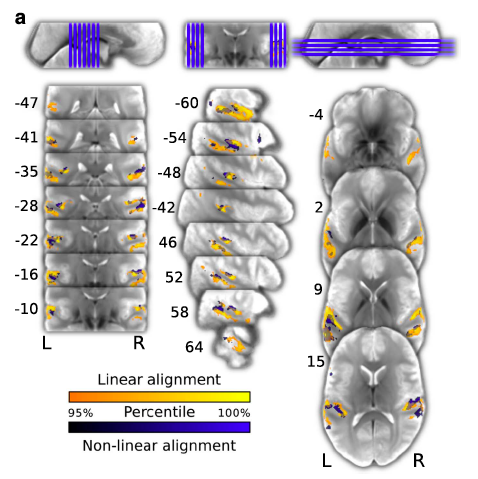
\includegraphics[height=8cm]{hanke_temporal_cortex.png}                            
\end{figure}  

\subsection{Discussion}
According to Hanke et al., the region that appeared to be highly similar 
between individuals in this study in both our analysis and theirs, the Planum Temporale, is known to be involved in 
` `processing complex sounds and speech,"\cite{hank2014audiomovie} such as one 
might hear while listening to an auditory movie.  Other studies besides 
Hanke et al.'s affirm that the areas we saw with the highest inter-subject
correlation appear to be activated by complex auditory stimuli\cite{chevillet2011functional}.

We have a few hypotheses as to why our correlation coefficients are 
higher than those reported by Hanke et al.  1) We used 
different motion-corrected data: they used a bandpass filter, while we 
used the preprocessed data provided by Poldrack and the OpenfMRI project group, which used a high-pass
filter.  2) We used a Gaussian filter to smooth the data; they do not 
indicate using any filter to smooth the data in their paper.  Smoothing 
spatially should increase the correlation between subjects, possibly 
explaining why our correlations are all higher than theirs.  3) We 
took the average of the correlation for each run to account for the runs
effect; they did not.  However, we expect that taking the average of 
the correlation for each run would lower the overall correlation, so
this hypothesis is not supported by our data, where our correlations
are higher than all of theirs.   4) We only used 5 subjects instead of
18.  The number of subjects should not make the correlation coefficients
higher or lower, but using different data undoubtedly makes the
correlation coefficients different.  5) Their correlations may be incorrect.
The values they reported for mean correlation coefficients in their 
written text of the paper do not line up with the values they report in 
their table.  For example, Hanke et al. reports the mean correlation 
coefficient values at the 95\% level as r = 0.076 (linear) and r = 0.078 
(non-linear) at the supplemental table shown online here: \href{http://www.nature.com/articles/sdata20143/tables/5}{Voxel-wise Inter-individual Correlation Table}, and r = .077 (linear) 
and r = .086 (non-linear) in the paper.  We contacted Hanke via Github issue, and he acknowledged 
the discrepancy, but has yet to get back to us on which is the correct value.  

A future study could run pairwise correlations between all 18 subjects and compare 
those values to that of Hanke et al.  These differences from Hanke et al.'s study suggest that changes such as those mentioned above can have an impact on the final
result, and it is incredibly important to think through all decisions in scientific
research.  

\section{Classification}

In addition to reproducing Hanke et al.'s analysis, we also wanted to
conduct our own, based on personal interest and ability.

After perusing all the stimulus-related data (e.g. data annotating each 
\emph{Forrest Gump} scene and when a subject was exposed to that scene), we 
decided to guide part of our analysis to see if we could
summarize any interesting trends in fMRI response with respect to these
features. We selected a single subject, Subject 1, to perform classification
upon, since we are interested on if it is possible to classify volumes in
general, without investigating the question of whether it is possible to 
classify volumes across individuals.

We used this information and the fMRI data to select features with the goal of
building the best possible predictor of certain aspects of a movie scene given
fMRI data. We wanted to be able to accurately predict whether a particular
movie scene falls under one of two categories: interior or 
exterior.  Our plan of action was to 1) select voxels that seemed to differ most 
between the two groups as features, and 2) use machine learning to classify 
volumes as belonging to one of two groups (i.e. interior or exterior).

\subsection{Classification of Interior/Exterior}

\subsubsection{Feature Selection}

To select voxels as features for our classification problem, we first
determined which volumes corresponded to parts of the movie that took place 
indoors (interior) and which volumes corresponded to parts of the movie that took place 
outdoors (exterior), using the scenes.csv file provided by Hanke et al., as 
described in the data section, and added that as a column in our design matrix. 
In order to account for baseline BOLD and any linear drift created by the subject 
moving in the scanner, we also included those two regressors in the design matrix.
Thus, our design matrix has 3 columns: a column of 
ones for the intercept, linear drift, and the boxcar function for our column of interest: interior (0) or exterior (1).

We then performed a t-test for each voxel to determine if the BOLD signal is
significantly different between interior volumes and exterior volumes.  Our null 
hypothesis is that there is no difference between interior and exterior volumes.
This gave us an array of t-statistics, one for each voxel, a total of 1,108,800.
We took the absolute value of the t-statistics because are only interested in
if the voxel has a different BOLD signal than 0, not whether it is higher or 
lower than expected. Since we wanted to select the voxels with the biggest 
change between groups (i.e. the largest t-statistics), we cut down that
number by selecting the top portion of them.  This number of feature
selections is rather arbitrary, but should be relatively small so we can
create a random forest that does not overfit.  Part of our analysis is
determining the optimal number of features to select. This will be done via
cross validation.

Because we are ultimately interested in feature selection, not in whether
certain voxels are significantly different between the two groups, we did not
correct for multiple comparisons.  If we were interested in the significance
of certain voxels, we would apply a Bonferroni correction.

We wanted to know which areas of the brain seemed to be most inclined to pick
up on the difference between interior and exterior scenes.  Thus, we plotted the 
betas testing the hypothesis that there is no difference in BOLD signal between 
interior and exterior volumes for each voxel.  Unfortunately, this looks very similar to our linear drift image, where there appears to be an artifact.


\subsubsection{Random Forest}

To see if we could predict whether a slice was taken from a day or night
scene, we focused on creating a random forest, using voxels selected in the 
feature selection step as the nodes.  We first trained on a random 80\% of the 
slices, collapsing day slices and night slices together, so that the distribution of
the slices selected was roughly equivalent to the distribution of the entire
data, rather than selecting 80\% of the day slices and 80\% of the night
slices.  The other 20\% of the slices we preserved to be our testing set.  We
created a decision tree, which we used to predict whether each slice in the
testing set took place during the day or the night.  In theory, we could use
the first six runs as the training set, and see how well they predict the last
two runs for a given participant.

\subsubsection{Results}

\begin{table}[H]
  \centering
  \caption{Cross-validation Accuracies}
  \label{tab:table3}
  \begin{tabular}{cc}
    Number of Features & CV Accuracy\\
    \hline
    500 & 0.9155\\
    \hline
    1000 & 0.91480\\
    \hline
    2500 & 0.9211\\
    \hline
    5000 & 0.9259\\
    \hline
    10000 & 0.9288\\
    \hline
    20000 & 0.9277\\
    \hline
    30000 & 0.9259\\
    \hline
    40000 & 0.9314\\
    \hline
    42000 & 0.9310\\
    \hline
    44000 & 0.9314\\
    \hline
    46000 & 0.9336\\
    \hline
    48000 & 0.9299
  \end{tabular}
\end{table}

The optimal number of features appears to be 4600, since that results in the 
highest cross-validation accuracy, 93.36\%.  Since random forest is a stochastic 
algorithm, reproducing this table will result in similar, but slightly different
cross-validation accuracies.

Seventy-seven percent of the volumes took place outside, so if the random forest
predicted outside for all volumes, it would have a prediction accuracy of 77\%
by random chance.  Thus, our random forest with 46000 features is performing much
better than random chance.

\subsection{Discussion}
Our classification analysis indicates that it is possible to predict whether a 
scene takes place inside or outside based on brain state.  We looked at random volumes throughout the 2-hour scan of one individual.  Future studies could investigate if it is possible to train upon one subject 
to classify volumes from other subjects.

Since day/night is also binary, we could apply the same methods to classify volumes
as taking place during the day or during the night.  We could also extend the 
analysis to predicting something not binary, like sentiment: positive, negative, or
neutral.

Future studies could take the voxels we selected to be feature selectors here, and
from classifications like the day/night or positive/negative/neutral analyses mentioned previously, and see if it is possible to distinguish individuals on the nature of those three regressors of interest.  For example, since the 20 participants have differing amounts of exposure to \emph{Forrest 
Gump}, with some participants having never seen the movie before and one 
participant who had seen the movie 12 times before, perhaps a future study could 
distinguish between individuals who are ` `familiar" with \emph{Forrest Gump} and individuals who are not using those three regressors of interest (i.e. interior/exterior, day/night, positive/negative/neutral).  However, there
are a relatively small number of participants, only 20, since fMRI is
expensive, so the predictive ability of that study would be rather limited.

\section{Conclusion/Overall Discussion}

\subsubsection{Interpretations and Implications}

Hanke et al. specifically only used free, open-source software and was very 
transparent about his data and methods to facilitate 
replications and further research by future investigators\cite{hank2014audiomovie}.  We did attempt to make our code and project as reproducible as
possible; however, we ran our analyses on Amazon and had to pay around \$100
for it.  Additionally, we only used five subjects for our reproduction analysis,
and only one subject for our classification analysis, due to the size of the data
and computational power available to us.  Thus, just as the size of the data presented a significant barrier to us, so might the size of this data present a 
barrier to the future work Hanke et al. desire to see using this dataset.

However, despite our use of only part of the data, we were still able to conduct
two analyses.  So perhaps Hanke et al. have succeeded in their goal of seeing 
future work arise from this dataset, although of a limited nature.

\bibliography{project.bib}

\end{document}

